\cotefile{156-3}
\scanpage{2}
\mspage{1}

\uline{Réseaux}\ldots\ via découpages.

(8 Juin 86)

% slanted; within the drawn corner enclosure
\margin{\figure{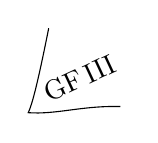
\begin{tikzpicture}[scale=.65]
\draw (.05,1.65) .. controls (-.10,.90) and (-.25,.20) .. (-.35,0) .. controls (.20,-.04) and (.70,.14) .. (1.45,.12);
\node[rotate=25] at (.65,.67) {GF\,\uline{III}};
\end{tikzpicture}}}

% slanted
\margin{\deleted{Ensembles} Parties \unsure{finies} de lieux \unsure{modérés|modérées}}

Je voudrais définir une autre axiomatique des \deleted{réseaux,}
\deleted{\unsure{l}}\unsure{la|a} structures de réseaux
sur un ens. $\mathcal L$ (\deleted{\unsure{d}}ens. des ``lieux'').

\textcircled{\scriptsize a}\quad $S_0\deleted{\unsure{(L)|L}}\subset P_2(L)$ l'ens des \uline{0-sphères}
\uline{plongées}, ou des \uline{paires} \deleted{\unsure{mod.}} (de
lieux) modérées. \inserted{si $\{a,b\}\in S_0$ ; on dit aussi que $a,b$ st \uline{disjoints} ou en position relative modérée.}

% slanted
\margin{Mais, on dit aussi que $a,b$ en position rel. modérée si $a=b$ \uline{ou} $\{a,b\}\in S_0$}

[En termes de l'axiomatique par les segments,
\unsure{cela|celà} signifie que \deleted{$a,b$ \unsure{sont} ou bien} \inserted{(à part $a,b$ \uline{distincts}},
\unsure{contenu} dans $\{a,b\}\in\deleted{\unsure{S_0}}P_2(\mathcal L)$, que
ou bien $\{a,b\}\cap\mathcal L_s\ne\varnothing$ ($a$ ou $b$ est un
nœud \unsure{sg$_r$|sg} du réseau) \uline{ou} \uline{bien} \deleted{$a,b$}
(si \deleted{\unsure{st|sont}} \inserted{$a,b$} réguliers) que $a,b$ \inserted{\unsure{doivt|doit}} \unsure{appartiennent|appartient} :
des lignes différentes, \unsure{soit|sont}, s'ils sont
dans une $\bar{=}$ ligne, que $\{a,b\}=\partial I$,
pour $I\in S$].

\deleted{\unsure{b)}} Une partie \uline{finie} \inserted{$T$} est dite \deleted{admissible} \inserted{``\uline{modérée}''}
si \deleted{$\forall\,a,b\in T$, \unsure{on a} $a,b$} $P_2(T)\subset S_0$
i.e. deux éléments quelc. de $T$ sont en
position relative modérée (\deleted{des} 2 à 2 ``disjoints'').

% paper watermark; faint outline impression
\rotatebox{90}{\textsc{\unsure{xtra Strong Ext}}}
\scanpage{3}
\mspage{2}

\deleted{De plus, on veut que la structure implique}

\deleted{\textcircled{\scriptsize b}\quad $\forall\,T\in P_{f\,\mathrm{mod}}(\mathcal L)$, on se donne une
relation d'équivalence $R_T$ dans l'ens
\unsure{où}}

Si $T$ est une partie finie
modérée\unsure{,|;}, on \deleted{\unsure{désignera|désigne} par} \inserted{pose}

\[
 C\deleted{\unsure{\mathrm{omp}^{r}|\mathrm{omp}}}_{\mathcal L}(T)=
 \{\,t\in\mathcal L\setminus T\mid \{T\cup\{t\}\}\ \text{\unsure{modéré|modérée}}\,\}
\]

% slanted
\margin{\uline{le complémentaire} \uline{modéré} de $T$.
Question : $T$ est-il connu quand on \unsure{connait|connaît} $C_{\mathcal L}(T)$ ? Plus précisément,
si $T'\subset T$, on a $C(T)\subset C(T')$, l'inverse est-il vrai ? Oui,
Donc, si \inserted{$t\in T'$} $t\notin T$, \deleted{\unsure{$t$ est gén.} \unsure{tel} ($T\cup\{t\}$ modéré) \unsure{puisque} \unsure{on a toujours} \unsure{$s\notin T$,}} alors $t\in C(T)$ et $t\notin C(T')$}

ou mieux, l'ens des $t\in L\setminus T$ en
position modérée p.r. à $T$.

[\uline{NB}\quad deux parties finies modérées
sont dites en position relative
modérée si leur-réunion est
modérée ; $t$ est dit en pos. rel.
modérée p.r. à $T$ si $\{t\}$ l'est ;
$s$ et $t$ sont dits en pos. rel. modérée
si $\{s,t\}$ est modéré i.e. \deleted{\unsure{si}},
$s\ne t$ ou $\{s;t\}\in S_0$ \ldots\ ]

% slanted
\margin{\uline{NB} $T$\deleted{\unsure{est}} est connu quand on \unsure{connait|connaît} $C(T)$}

\textcircled{\scriptsize b}\quad $\forall\,T\in\underbrace{\mathrm{Modf}}_{\substack{\text{parties mod}\\\text{finies}}}(\mathcal L)$, une relation
d'équivalence $R_T$ dans $C_{\unsure{\checkmark|\mathcal L|}}(T\unsure{)|\}}$ (dont
les classes s'appellent les \uline{comp. connexes} \inserted{de $C(T)$}

% paper watermark, visible from the reverse
\rotatebox{90}{\textsc{\unsure{xtra Strong Ext}}}
\scanpage{4}
\mspage{3}

\textcircled{\scriptsize c}\quad $\forall\,T\in\mathrm{Modf}(\mathcal L)$, et $A\in C(T)/R_T$
une classe suivant $R_T$, une partie
de $\dot A\subset T$, appelée \uline{frontière} de $A$.

Ces données \textcircled{\scriptsize a} \textcircled{\scriptsize b}, \textcircled{\scriptsize c} étant \unsure{assujetties}
à satisfaire certains axiomes.

Je prévois que les axiomes impliquent
\deleted{Soit \illegible{1} $\unsure{t|U}\in C(T)$, \unsure{on pose}}
ceci

1°) que la donnée \textcircled{\scriptsize c} résulte déjà de \textcircled{\scriptsize b}

2°) que la donnée \textcircled{\scriptsize b} résulte de
la donnée des $R_T$, \deleted{\unsure{pour}} dans le cas
particulier où $T\in S_0$. Donc
les seules \unsure{donnée|données} essentielles \unsure{serait|seraient}
\textcircled{\scriptsize a} \unsure{celles|celle} des 0-sphères i.e. la notion
de \deleted{pos.} lieux en pos. relative modérée
(condition \inserted{réflexive et} symétrique) et \textcircled{\scriptsize b} La donnée,
pour \figure{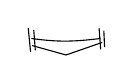
\begin{tikzpicture}[x=1cm,y=1cm,baseline=-.4ex]
\draw (0,.12)--(.03,-.18) (0.07,.10)--(.09,-.16);
\draw (.90,.12)--(.92,-.15) (.96,.09)--(.97,-.12);
\draw (.04,-.01) to[out=-8,in=187] (.92,-.01);
\draw (.05,-.10)--(.48,-.22)--(.94,-.06);
\end{tikzpicture}} $\varepsilon\in S_0$, de la relation
d'équivalence $R_{\varepsilon}$ dans $C(\varepsilon)$.

\deleted{On va} \uline{Axiomes provisoires :}

\deleted{Soit $X$} Appellons les $U$ de la forme
$C(\deleted{\unsure{L}}T)$ \uline{parties modérées cofinies}. On

% paper watermark
\rotatebox{90}{\textsc{\unsure{Strong Extra St}}}
\scanpage{5}
\mspage{4}

veut que si $U$ \deleted{$(=C\unsure{)(|(}T)$} est à la fois modéré fini
et modéré cofini, donc si $S$ et $T$
sont \deleted{deux} parties modérées finies
\deleted{telles} disjointes telles que \deleted{\unsure{tout}} \inserted{a)} $S\cup T$
modéré i.e. \figure{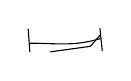
\begin{tikzpicture}[x=1cm,y=1cm]
\draw (0,.16)--(.02,-.13) (.91,.17)--(.94,-.12);
\draw (.01,-.02) to[out=0,in=197] (.92,.04);
\draw (.28,-.13)--(.79,-.06)--(.91,.08);
\end{tikzpicture}} $\unsure{s|S}\in S$ modéré p.r. à tt
$t\in T$, et b) Tout $u\in\mathcal L$ \unsure{modér.|modéré} p.r. à
$S$ est dans $T$\unsure{;|,}, \deleted{alors $S\cup T=\mathcal L$} et
à fortiori $S\cup T$ est partie \inserted{finie} modérée
maximale, donc $S\cup T=\mathcal L$, et
$\unsure{{}^{\cdot\cdot}S_0|S_0}=P_2(\mathcal L)$, enfin les relations
d'équivalence sont discrètes, et les
$\dot A$ sont vides. Pour le formuler,
on définit \unsure{la|a}

\deleted{Déf} \inserted{Ex 1} \uline{structure \inserted{de Réseau} discrète} sur $\mathcal L$

\[
 S_0=P_2(\mathcal L)\ \Longrightarrow\
 \left\{\begin{aligned}
 &\mathrm{Modf}(\unsure{\mathcal L|\mathcal L_0})=\deleted{\unsure{\mathrm{Mod}}}P_f(\mathcal L)\\
 &C_T=\mathcal L\setminus T\qquad\text{si }T\in P_f(\mathcal L)
 \end{aligned}\right.
\]

\[
\begin{aligned}
 &\deleted{C(T)=\unsure{\subset|\mathcal L}}\\
 &R_{\unsure{T|T\rceil|\Pi}}=\text{relation d'équivalence discrète}\\
 &\hspace{3em}\text{dans }\mathcal L\setminus T,\quad\text{donc les composantes}\\
 &\hspace{4em} \inserted{A}\ \text{sont réduites à un pt}\\
 &\deleted{\text{Pour Donc}}\\
 &\dot A=\varnothing
\end{aligned}
\]

\uline{Axiome}\quad Si $T$ est partie finie modérée
maximale, alors $T=\mathcal L$, $\mathcal L$ est \unsure{discrêt|discrèt|discret}.

% paper watermark, visible from the reverse
\rotatebox{90}{\textsc{\unsure{Strong Extra St}}}
\scanpage{6}
\mspage{5}

On va faire des hyp.thèses de
finitude \unsure{draconniennes|draconiennes}, peut-être
provisoires

% slanted
\margin{Finitude}

$\underline{\mathrm{Dec}}_1$\quad \deleted{\unsure{l}}l'ens des comp. connexes
de tout $U$ est \uline{fini}.

\deleted{\uline{Définition} Partie modérée \uline{fermée}}

$\underline{\mathrm{Dec}}_2$\quad \unsure{Soit|Soient}\deleted{\unsure{ent}} $U$\inserted{$=C(\deleted{\unsure{T}}S), V=C(\deleted{\unsure{S}}T)$} \unsure{partie|parties} modérée
cofinies, avec $U\subset V$ i.e. $T\subset S$.
Alors tte composante connexe \inserted{$A$} de
$U$ est contenue dans une comp.
connexe (unique bien sur) $B$ de $V$.

De plus, on a

\diagram{\begin{tikzcd}[ampersand replacement=\&,row sep=0.35ex,column sep=0.4em,
cells={nodes={inner sep=1pt}},execute at end picture={
\draw[line width=.35pt] ([yshift=-.2ex]aa.south west) to[out=-90,in=180] ([xshift=.3ex,yshift=-.55ex]aa.south west) -- ([xshift=-.3ex,yshift=-.55ex]aa.south east) to[out=0,in=-90] ([yshift=-.2ex]aa.south east);
\draw[line width=.35pt] ([yshift=-.2ex]bb.south west) to[out=-90,in=180] ([xshift=.3ex,yshift=-.55ex]bb.south west) -- ([xshift=-.3ex,yshift=-.55ex]bb.south east) to[out=0,in=-90] ([yshift=-.2ex]bb.south east);
}]
|[alias=aa]| \dot A \& \cap\,T\,\subset \& |[alias=bb]| \dot B\\
\cap \& \& \cap\\
\unsure{s|S} \& \& T
\end{tikzcd}}

% paper watermark; read from foot to head; clipped at the two sheet edges
\rotatebox{90}{\textsc{\unsure{t}rong Extra Str}}
\scanpage{7}
\mspage{6}

\uline{Ex \deleted{\unsure{1}}2}\quad Soit $\deleted{\unsure{S|E}}$ $\mathcal L$ un ens ordonné,
on suppose $\mathcal L$ filtrant croissant, filtrant
décroissant, sans plus grand ni
plus petit \unsure{élémt|élément}, loc. filtrant croissant
et filtrant décroissant, divisible.

On appelera un tel ensemble une
\uline{ligne ordonnée}

\[
S_0\subset P_2(\mathcal L)\qquad
\deleted{\text{Soit }\{x,y\}\in P_2(\mathcal L)}
\]

\textquotedbl\quad \unsure{partie|parties} \deleted{qui} de card. 2 \deleted{\unsure{une}} qui sont \uline{tot.} ordonnées

\[
\begin{aligned}
&\mathrm{Modf}(\mathcal L)=\text{parties finies tot ordonnées}\\
&\hspace{8em}\deleted{\text{i.e. telles que}}
\end{aligned}
\]

\[
\begin{aligned}
 \text{Soit }T\in\mathrm{Modf}(\mathcal L),\qquad &T=\{t_{\unsure{p|1}},t_2,\ldots,t_{n}\}\\
 &\quad t_1<\unsure{t|l|1}_2<\ldots<t_n
\end{aligned}
\]

Alors les composantes connexes sont

\[
\underbrace{\mathopen{]}-\infty,t_1\mathclose{[}}_{t_1},\
\underbrace{\mathopen{]}t_1,t_2\mathclose{[}}_{t_1,t_2},\
\ldots\quad
\underbrace{\mathopen{]}t_{n-1},t_n\mathclose{[}}_{t_{n-1}\,t_n},\
\underbrace{\mathopen{]}t_n,\infty\mathclose{]}}_{t_n}
\]

% slanted
\margin{Pts frontière}

($n+1$ composantes connexes)

% paper watermark; mirror impression across the letters
\rotatebox{90}{\textsc{\unsure{t}rong Extra Str}}
\scanpage{8}
\mspage{7}

Cette structure ne change pas si
\deleted{\unsure{de}}on change l'ordre par ordre opposé,
i.e. elle ne dépend que du
biordre.

\deleted{Partie modérée} \deleted{\unsure{Segments|Segment}}

% slanted
\margin{refaire, sans se borner à une ligne : sous tronçon fermé d'un tronçon. C'est un tronçon \unsure{p.|pour} le biordre induit. D'autre part, le bord d'un tronçon est défini Comme des}

\unsure{Tronçons|Tronçon} de la ligne : parties
de la forme

\[
\left\{\begin{aligned}
 &[s,t] &&s\leq t\\
 &\mathopen{]}-\infty,s],\quad\text{ou}\quad [s,+\infty\mathclose{[}\\
 &\mathcal L=\mathopen{]}-\infty,+\infty\mathclose{[}
\end{aligned}\right.
\]

Bord du tronçon : $\{s,t\}$ dans le
premier cas, $\{s\}$ dans le second, $\varnothing$ \inserted{troisième}

Deux tronçons sont dits en
position relative modérée, si leurs
bords : le sont.

\uline{Partie} \uline{modérée} :
réunion \inserted{finie} de tronçons \inserted{en position} mutuelle
modérée, et disjoints. \deleted{Donc} Par
définition, son bord est la réunion
(disjointe) des bords.

% paper watermark; clipped at the two sheet edges
\rotatebox{90}{\textsc{\unsure{r}ong Extra Stro}}
\scanpage{9}
\mspage{8}

\deleted{\uline{Proposition}}

\deleted{\uline{Définition} $\overbrace{\text{Segment, intervalle, demi-intervalle}}^{\inserted{\text{tronçons}}}$
(comme structure de réseau).}
\deleted{Segment}

\uline{Définition}\quad Un ens. ordonné \inserted{$\mathcal L$} est appelé un \uline{tronçon} \uline{ordonné} si

\unsure{a}) $\forall\,a\in\mathcal L$ tel que $\mathcal L_{>a}\deleted{\unsure{\sim|=}}\unsure{\ne|=}\varnothing$, $\mathcal L_{>a}$ est filtrant décroissant
\deleted{i.e. $\forall\,x,y$ $\unsure{a|x},y$ tels que} \inserted{si $a,y,\unsure{a|x}\in\mathcal L$ tels que}
$a>a$, $y>a$ alors $\exists\,z\in\mathcal L$ avec $x,y\geq z>a$

$\deleted{\unsure{b|a}}a'$) Axiome dual : si $a,x,y\in\mathcal L$ tels q
$\unsure{x|a}<a$, $y<a$ alors $\exists\,z\in\mathcal L$ avec $a,y\leq z<a$

b) $\mathcal L$ est filt\unsure{ant|rant} croissant et filtrant décroissant i.e.
$x,y\in\mathcal L\Rightarrow\exists\,a,b\in\mathcal L$ avec $a\leq x,y\leq b$

c) Si $x,y\in\mathcal L$ tels que $x<y$, $\exists\,z$ tel que $x<z<y$ .

d) $\deleted{\mathcal L\,\unsure{\ne|=}}$ $\operatorname{Card}\mathcal L>1$ \deleted{\unsure{(imp.|(}}

% slanted
\margin{\uline{NB} les cond $a\ a'\ b)\ c)$ sont satisfaites si $\operatorname{card}\mathcal L\leq1$ !}

On dit que $\mathcal L$ est un \uline{segment} si de plus $\mathcal L$ admet un plus petit et
\deleted{\unsure{(p.|(}} un plus grand élément, un \uline{intervalle} s'il n'admet ni l'un ni l'autre,

% paper watermark, visible from the reverse
\rotatebox{90}{\textsc{\unsure{n}g Extra Stro}}
\scanpage{10}\mspage{9}
% ink top, lines 1–3
un \uline{demi}-\uline{intervalle} s'il admet un plus petit élément mais pas un plus grand, ou bien l'inverse.

% ink upper middle, NB, lines 1–4
\deleted{\unsure{L'opposé|L'oppo}}\inserted{\uline{NB}} L'opposé d'un tronçon, segment, intervalle, demi-intervalle est itou. L'opposé d'un $1/2$ intervalle fermé à g. est fermé à droite, et inversement.
% ink left, slanting upwards beside NB
% slanted
\margin{Dans ma actuelle terminologie, tronçon \unsure{est|être|était|etre} \unsure{``ens|ens|un|équiv} \uline{biordre}}

% ink middle, Tout, lines 1–3
\deleted{\unsure{Lorsque|Lorsqu.}}\inserted{Tout} tronçon est l'un des trois (segment, $1/2$ intervalle, intervalle) à l'exclusion des deux autres.

% ink lower middle, Si L
Si $\mathcal L$ est un tronçon, on pose $\deleted{\unsure{\partial L}=}$
\[
\begin{aligned}
\unsure{\partial|\partial L}&=\bigl\{\,x\in L\mid
\begin{aligned}&x\text{ est plus petit élément}\\
&\text{ou plus grand élément}\end{aligned}\,\bigr\}
\end{aligned}
\]
\deleted{\illegible{1}}

% ink bottom, Soit and first equality
Soit $\mathcal L$ un tronçon, et
\[
\begin{aligned}
S_0(\mathcal L)=\mathrm{Drap}_2(\mathcal L)&=\{\,\unsure{\varepsilon|\mathcal E|E}\in P_2(\mathcal L)\mid \unsure{\varepsilon|\mathcal E|E}\text{ tot ordonné}\,\}\\
&=\{\,\{x,y\}\mid x<y\,\}
\end{aligned}
\]
% ink bottom, final equality
\[
\text{D'où}\qquad \mathrm{Modf}(\mathcal L)=\mathrm{Drap}(\mathcal L)
=\{\,S\subset P_f(\mathcal L)\mid S\,\substack{\text{tot}\\\text{ord}}\,\}
\]

% pale vertical paper watermark, rotated for reading
\rotatebox{90}{\textsc{\unsure{ra} Strong Extra}}
\scanpage{11}\mspage{10}
% ink top, Si S and C(S)
Si $S\in\mathrm{Modf}(\mathcal L)$, on a donc $\deleted{C(S)=}$
\[
C(S)=\{\,\deleted{\unsure{s|x}}t\in\mathcal L\mid\deleted{\unsure{S\cup\{t\}}}\ t\notin S,\quad S\cup\{t\}\ \text{tot. ord}\,\}
\]

% ink upper third, On a dit
On a dit comment on décomposait en ``composantes connexes'' un $C(S)$ \unsure{où|à|.}
\[
 S=\{s_{\unsure{p|1|0}},\ldots s_n\},\qquad s_{\unsure{p|1|0}}<s_2,\!<\cdots<s_n\,.
\]
Les comp. connexes sont les ens non vides parmi
\[
\mathcal L_{<s_{\unsure{p|1|0}}},\quad \deleted{\unsure{L}}[s_{\unsure{p|1|0}},s_2],\quad\ldots,\ [s_{n-1},s_n],\quad \mathcal L_{>s_n}
\]
% ink middle, bracketed cases
\[
\begin{aligned}
\bigl[\quad&\text{cas }n=0:\quad\text{une seule comp. }\mathcal L\\
&\text{\unsure{en|cas} }n=1:\quad\deleted{\text{\unsure{une}}}\ \text{deux composantes}\quad \mathcal L_{<s},\ \mathcal L_{>s}\\
&\hspace{7em}\text{(celles qui sont non vides)}\\
&\text{cas }n\geq2:\quad\text{voir \unsure{la|le|ce} \unsure{suite|suit} plus haut}\quad\bigr]
\end{aligned}
\]
% ink below cases, two extreme components
les seules non vides éventuelles étant $\mathcal L_{<s_1}$ (\inserted{si} $s_1$ plus petit élément) et $\mathcal L_{>s_n}$ (\inserted{si} $s_n$ plus grd élément). Les bords \deleted{sont} respectivement
% ink lower third, bords
\[
\underset{\substack{\rule{.4pt}{.6ex}\rule{4.8em}{.4pt}\rule{.4pt}{.6ex}\\\text{si comp. existe}}}{\{s_1\}\ \substack{\deleted{\unsure{s_1}}\\\deleted{\unsure{\text{donc }\varnothing}}\\\deleted{\unsure{\varnothing}}}},
\quad\{s_1,s_2\},\quad\ldots,\quad\{s_{n-1},s_n\},\quad
\underset{\substack{\rule{.4pt}{.6ex}\rule{2.7em}{.4pt}\rule{.4pt}{.6ex}\\\text{si comp. existe}}}{\{s_n\}}
\]

% ink bottom, Je dis
Je dis que l'on récupère la structure dé \deleted{\unsure{ordr|ordre}} biordre du tronçon (donc aussi la structure \textcircled{a}. \textcircled{b} \textcircled{c}) en termes de la seule structure \textcircled{a}, $+$ \textcircled{b} pour $T\in\unsure{\mathscr S|S}_0$.

% pale watermark seen through the paper
\rotatebox{90}{\textsc{\unsure{ng Extra Stro}}}
\scanpage{12}\mspage{11}
% ink opening line
Pour ceci, on note \deleted{\unsure{qu'une str}}\inserted{d'abord}

% ink Lemme, first four lines
\uline{Lemme} Une structure de \deleted{biordre} tronçon biordonnien est connue quand on connaît la relation en \deleted{$\{a,b,c\}$} trois \unsure{élémt|éléments} $a,b,c$
% ink relation R, first display
\[
\begin{aligned}
\left.\vphantom{\substack{X\\X}}\right|\!\left.\vphantom{\substack{X\\X}}\right|\!\left.\vphantom{\substack{X\\X}}\right|\, R(a,b,c)
&\qquad b\ \text{\uline{est strictement entre}}\\
&\qquad\qquad\text{\uline{$a$ et $c$}}
\end{aligned}
\]
(au sens que $a<b<\deleted{\unsure{e}}c$ \uline{ou} $a>b>c$)
% ink left, short diagonal note beside the three strokes
% slanted
\margin{relation sym. en $a,c$}
% ink left, NB, diagonal block
% slanted
\margin{\uline{NB} \deleted{\unsure{On a de}}\inserted{La conn. de} Cette relation $R$ implique la relation $\bar R$ non stricte \deleted{\unsure{($a=b=c$} \unsure{ou}}\ \deleted{$\unsure{a=b<c}$}\ $a\leq b\leq c$ ou $a\geq b\geq c$ \deleted{$\unsure{a\leq b\leq c}$} $(\unsure{\rightleftarrows|\Leftrightarrow})$ \deleted{$\{a,b,c\}$} $b$ entre $a$ et $c$ \inserted{\uline{strict}} ou $\{a,b,c\}$ est un drapeau de cardinal $\leq 2$}

% ink middle, Dém and équivalence
\uline{Dém} \deleted{Choisissons} On en déduit la relation (i.e. \inserted{la conn. de} $S_0(\mathcal L)$\deleted{\unsure{)}} i.e. de $\mathrm{Drap}(\mathcal L)$)
\[
\begin{aligned}
\deleted{\unsure{a}}\,a\text{ et }b\ \text{``disjoints''}\quad&
\text{i.e. distincts et comparables}\\
&\text{(i.e. }\{a,b\}\in\mathrm{Drap}_2(\mathcal L)\\
&\text{pour le biordre}
\end{aligned}
\]
% ink lower middle, formule ssi
par 
\[
\begin{aligned}
a\text{ et }b\ \text{disjts}\quad \text{ssi}\quad
\exists\,c\ \text{tel que }c\text{ entre}\\
a\text{ et }b
\end{aligned}
\]
(utilise divisibilité ! d\deleted{\unsure{es}}\unsure{u} \deleted{\unsure{drap. le ré}} biordre)

% ink bottom, Choisissons
\deleted{\illegible{1}} Choisissons $\unsure{\varepsilon|\mathcal E|E}\in S_0$ (existe, car \deleted{si $x,y\in$} par hyp $\exists\,x,y\in\mathcal L,\quad x\ne y$, donc $a\leq x,y\leq b$, et on a $a\leq b$ et $a\ne b$ \deleted{\unsure{)}} \deleted{\unsure{c|p}}car sinon on aurait $x=y$)
% ink lower left, four short oblique lines
% slanted
\margin{Il existe $=$ des \unsure{drap.} de long. arbitraire}

% pale vertical watermark
\rotatebox{90}{\textsc{\unsure{ra Strong Extra}}}
\scanpage{13}\mspage{12\unsure{..|.}}
% ink top, first two lines
et choisissons une ``origine'' $a$ dans $\unsure{\varepsilon|\mathcal E|E}=\{a,b\}$ (ce qui va déterminer la relation d'ordre).

% ink upper third, Considérons
\deleted{Soit} \deleted{Alors} Considérons sur $\mathcal L$ la relation d'ordre définissant le biordre, telle que $a<b$. On va voir qu'elle est \unsure{entièmt|entièrement} déterminée par la conn. \deleted{\unsure{de}}du \deleted{\unsure{la paire}}\inserted{couple} $(a,b)$

% ink upper middle, On aura, three defining sets
On aura \unsure{.}
% slanted
\margin{déterminés par $R$}
\[
\left\{\begin{aligned}
\mathcal L_{\deleted{\unsure{>}}\geq b}&=\{\,x\in\mathcal L\mid\deleted{x=b\text{ ou}}\ \inserted{x=b\text{ ou}}\ b\text{ entre }a\text{ et }x\,\}\quad\deleted{\unsure{a,b|a<b}.}\\
\mathcal L_{\leq a}&=\{\,x\in\mathcal L\mid\inserted{x=a\text{ ou}}\ a\text{ entre }\deleted{\unsure{a}}b\text{ et }x\,\}\\
\deleted{\unsure{\mathcal L}}\mathopen{]}\deleted{\unsure{x}}a,b\mathclose{[}&=\{\,x\in\mathcal L\mid x\text{ entre }a\text{ et }b\,\}
\end{aligned}\right.
\]
% ink left, below brace
% slanted
\margin{donc}

% ink middle, question
\deleted{Quand}\inserted{Soient} $u,v\in\mathcal L$, quand a-t-on
\[
u\leq v\qquad\unsure{\mathord{?}|.}
\]
Il faut et suffit qu'il existe
\[
\begin{aligned}
&\deleted{x\in}\quad x,y\in\mathcal L\quad\text{tels que}\\
&x\in\mathcal L_{\leq a},\ y\in\mathcal L_{\geq b}\qquad\text{et}\\
&\hspace{2em}x\leq u\leq v\leq y
\end{aligned}
\]
% ink bottom, i.e., left bracket
\[
\text{i.e.}\quad
\left[\begin{aligned}
&\deleted{\{\unsure{x},y,\unsure{u|b},v\}\ \text{est }\in\mathrm{Drap}(\mathcal L)}\\
&\qquad\deleted{x,y\in}\quad x\in\mathcal L_{\leq a},\ y\in\mathcal L_{\geq b}\quad(\text{donc }x<y)\\
&\deleted{\text{avec }x\text{ plus petit élément}}\\
&\deleted{u\text{ est entre}}\quad u,v\text{ sont entre }x\text{ et }y\\
&\quad u\text{ est entre }x\text{ et }v\qquad.\\
&\quad v\text{ est entre }u\text{ et }y
\end{aligned}\right.
\]

% pale vertical watermark
\rotatebox{90}{\textsc{\unsure{g Extra Stro}}}
\scanpage{14}\mspage{13}
% ink top, opening and lemma
Donc il faut simplement vérifier le

\uline{Lemme} Soit $\mathcal L$ un ens ordonné, et $x,y,u,v$ trois \unsure{élémts|éléments}, tels que
% ink upper third, clauses a–d and brace at right
\[
\begin{aligned}
&\text{a)}\quad u,v\text{ sont entre }x\text{ et }y\\
&\left.\begin{aligned}
&\text{b)}\quad u\text{ est entre }x\text{ et }v\\
&([\,\text{c)}\quad v\text{ est entre }u\text{ et }y\,]\deleted{\unsure{)}}
\end{aligned}\ \right\}\quad
\begin{aligned}&\text{une des deux}\\&\text{en suffit}\end{aligned}\\
&\text{d)}\quad x<y\quad,
\end{aligned}
\]
alors on a
\[
x\leq u\leq v\leq y
\]

% ink middle, Dém, first four lines
\uline{Dém} \deleted{\unsure{L'ass|L'assert}} \unsure{les|Les} conditions b) c) d) impliquent que $I\deleted{\unsure{\{x}}=\{x,y,u,v\}$ est un drapeau, \deleted{\unsure{Prouvons|Prenons}} et \unsure{SPG} $\mathcal L=I$ est un ens tot. ordonné \deleted{que $x$ en} à 2, 3, ou 4 \unsure{élémts|éléments}.
% ink middle, crossed proof and interlinear replacement
\deleted{Alors \unsure{Prouvons|Prenons}} \inserted{Comme $u,v$ sont} \deleted{que $x$ est le plus petit élément, donc (comme $x<y$) que l'on ne peut avoir $u<x$, ni $v<x$. Supposons $u<x$ ($<y$) ; comme $u$ est entre $x$ et $v$, on aurait \unsure{$v\leq u<$}\ $v<u<x<y$} \inserted{entre $x$ et $y$ et $x<y$,} on doit avoir $x\leq u,v\leq y$, \deleted{il reste à prouver $u\leq v$} et comme $u$ est entre $x$ et $v$, on doit avoir $x\leq u\leq v$\quad OK

% ink bottom, NB and lettered lines
\uline{NB} On a utilisé
\[
\begin{aligned}
&\text{a) la divisibilité de la rel. d'ordre}\\
&\text{b) le fait que }\mathcal L\text{ soit filtrant}\\
&\hspace{2em}\text{croissant et filtrant décroissant.}
\end{aligned}
\]
% ink last two lines
Et a) n'a servi qu'à montrer que la relation ``$a$ et $b$ disjoints'' est déductible de ``$a$ est str. entre $b$ et $c$''

% pale vertical watermark
\rotatebox{90}{\textsc{\unsure{g Extra Strong}}}
\scanpage{15}\mspage{14}
% ink top, relations
Si on se donne à la fois les deux relations
\[
\left\{\begin{aligned}
\unsure{\underline R|R}(a,b)&\qquad \{a,b\}\in\mathrm{Drap}_2(\mathcal L)\\
R(a,b,c)&\qquad b\text{ est str. entre }a\text{ et }c
\end{aligned}\right.
\]
alors pour récupérer le biordre, il suffit de supposer $\mathcal L$ filtrant croissant et filtrant décroissant, \deleted{et les relations \unsure{Si|si}, \unsure{Cet|cet|Oct} \unsure{sur les}, filtrant \unsure{cr.} et \unsure{décr.} \unsure{sont} de \unsure{qque|toutes} \unsure{comp.|faç.} \unsure{connexes|connues en} \unsure{$S_0$|$v_0$|$0$}} 

% ink middle, On va voir
\deleted{\unsure{On va}} On va voir maintenant comment la connaissance\inserted{ de $\mathrm{Drap}_2(\mathcal L)$, et} pour $\unsure{\varepsilon|\mathcal E|E}\in\mathrm{Drap}_2(\deleted{\unsure{I}}\mathcal L)$, de la décomp. de
% ink middle, C(\unsure{\varepsilon|\mathcal E|E}) and continuation
\[
 C(\unsure{\varepsilon|\mathcal E|E})=\{\,t\in\mathcal L\deleted{\unsure{\notin\varepsilon|\smallsetminus\varepsilon}}\mid
 \deleted{\unsure{x}}\{\unsure{\varepsilon|\mathcal E|E}\unsure{\cup|,}t\}\deleted{\unsure{=|-}}\in\mathrm{Drap}_3(\mathcal L)\,\}
\]
en composantes connexes, implique la connaissance de la relation
\[
 R(a,b,c)\unsure{\mathord{:}|\mathord{?}}\quad b\text{ strict entre }a\text{ et }c.
\]
% ink lower third, Première condition
Première condition : $\{a,b,c\}\in\mathrm{Drap}_3(\mathcal L)$ (résulte de la donnée de $\mathrm{Drap}_2(\mathcal L)$)
\figure{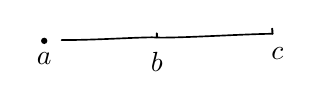
\begin{tikzpicture}[x=1cm,y=1cm,line cap=round]
\fill (0,0) circle (1.15pt);
\draw[line width=.6pt] (.22,.01) .. controls (.66,.01) and (1.06,.04) .. (1.37,.045) .. controls (1.61,.026) and (2.48,.085) .. (2.9,.09);
\draw[line width=.7pt] (1.43,.045) -- (1.43,.095) (2.9,.09) -- (2.895,.155);
\node[below] at (0,-.025) {$a$};
\node[below] at (1.43,-.015) {$b$};
\node[below] at (2.96,.035) {$c$};
\end{tikzpicture}}
% ink bottom, final sentence and cancelled display
Si $b$ est entre $a$ et $c$, regardons les
\[
 \deleted{J_{abc}=\text{composante de }C(\{a,b\}}\unsure{,|)}
\]

% pale vertical watermark
\rotatebox{90}{\textsc{\unsure{ng Extra Stro}}}
\scanpage{16}\mspage{15}
% ink top, heading of the three equalities
trois composantes (relatives à la \unsure{donné|donnée} de $\{a,b,c\}$)
\[
\begin{aligned}
\deleted{\unsure{C}}X_{\{a,b\}}&=\deleted{\unsure{C(a,b,c)}}=(\text{comp. de }C(\{a,b\})\text{ contenant }c)=\mathcal L_{>b}\\
X_{\{b,c\}}\deleted{\unsure{C(b,c,a)}}&=(\rule{1.45cm}{.4pt}\ C(\{b,c\})\ \rule{1.1cm}{.4pt}\ a)=\mathcal L_{<b}\\
X_{\{c,a\}}\deleted{C(c,a,b)}&=\rule{1.2cm}{.4pt}\ C(\{c,a\})\ \rule{.85cm}{.4pt}\ b)=\deleted{\unsure{\mathcal L}}\mathopen{]}a,c\mathclose{[}
\end{aligned}
\]

% ink middle, On trouve and three intersections
On trouve
\[
\begin{aligned}
&\deleted{C}X_{\{a,b\}\deleted{\unsure{c}}}\cap\deleted{C}X_{\{b,c\}\deleted{\unsure{a}}}=\varnothing\\
&\left.\begin{aligned}
&\deleted{C}X_{\{a,b\}\deleted{\unsure{c}}}\cap\deleted{C}X_{\{c,\deleted{\unsure{b}}a\}\deleted{\unsure{b}}}=\mathopen{]}b,c\mathclose{[}\ne\varnothing\\
&X_{(b,\unsure{c|b}\}}\cap X_{\{c,a\}}=\mathopen{]}a,b\mathclose{[}\ne\varnothing
\end{aligned}\right\}
\end{aligned}
\]
% ink right of the two nonempty intersections
\margin{divisibilité !}
% ink lower middle, donc b
donc $b$ est distingué, dans $J=\{a,b,c\}$, par la propriété que pour les deux \deleted{parties} ${\unsure{\varepsilon|\mathcal E|E}}',\unsure{\varepsilon|\mathcal E|E}'$ \deleted{de} $\in\unsure{P|\mathscr P|\mathfrak P}_2(J)$ qui le \unsure{contient|contiennent}, on a
\[
 X_{\unsure{\varepsilon_{0}|\varepsilon_{,}|\varepsilon}}\wedge X_{\unsure{\varepsilon|\mathcal E|E}'}=\varnothing\,.\qquad\text{On gagne !}
\]

% ink bottom, NB
\uline{NB} On a à nouveau utilisé la divisibilité.

% pale vertical watermark
\rotatebox{90}{\textsc{\unsure{ng Extra Strong}}}
\scanpage{17}\mspage{16}
% ink heading and first remark
\uline{Remarques} \textcircled{1} \deleted{\unsure{Considér|Considé}} sur la notion de tronçon. On cherche une sous-cat. pleine \inserted{$\mathscr T$} de celle des ens. ordonnés, satisfaisant

% ink item a, two lines and qualification at the right
a) \deleted{\unsure{S}}Tout $\mathcal L\in\mathrm{Ob}\,\mathscr T$ est filtrant croissant et filtrant décroissant, et \deleted{non vide} \inserted{de cardinal $\ne1$} (donc $\geq2$)

% ink item b
b) Si $x,y\in\deleted{\unsure{T}}\mathcal L_{\deleted{\unsure{,|g}}}\in\deleted{\unsure{O}}\mathrm{Ob}\,\mathscr T$, et $x<y$, $\exists$
\[
 z\in\mathcal L,\qquad x<z<y\qquad\text{(divisibilité)}
\]

% ink item c
c) Si $x\in\mathcal L\in\unsure{\mathrm{Ob}|\mathrm D}\,\mathscr T$, \deleted{alors} et si
\[
 \mathcal L_{>x}\ne\varnothing,\quad\text{alors}\quad \mathcal L_{>x}\in\mathrm{Ob}\,\mathscr T\,.
\]

% ink item c prime
c$'$) Dual de c)

% ink middle and lower third, Il y a
Il y a \unsure{une|un} plus \unsure{grande|grand} $\mathscr T$ qui satisfait ces conditions, et $\mathscr T$ est stable par passage à l'ordre opposé. Les objets de $\mathscr T$ sont les tronçons ordonnés.

% ink bottom, second remark
\textcircled{2} Il faudrait expliciter \unsure{quelle|quelles} \unsure{condition|conditions} la relation $R(a,b,c)$ doit satisfaire, pour définir une structure de \unsure{\deleted{tr.}}tronçon \unsure{biordonné|biordonnien}\unsure{,} et itou pour la donnée de $S_0\subset\unsure{P|\mathscr P|\mathfrak P}_2(\mathcal L)$ et les $R_{\unsure{\varepsilon|\mathcal E|E}}$\unsure{,} ($\unsure{\varepsilon|\mathcal E|E}\in S_0$) sur les $C(\unsure{\varepsilon|\mathcal E|E})$ \ldots

% pale vertical watermark
\rotatebox{90}{\textsc{\unsure{ng Extra Stro}}}
\scanpage{18}\mspage{17}
Sous tronçon \deleted{\illegible{1}}\inserted{fermé $I$} d'un tronçon $\mathcal L$ : sous ens. de la forme $[a,b]$ (avec $a<b$) ou $L_{\leq a}$ (avec $a$ pas le plus petit élément) ou $L_{\geq\deleted{\unsure{b}}a}$ (avec $b$ pas un plus grand élément), \inserted{ou $L$} : ce sont donc des tronçons, pour la structure de \unsure{biordre|biordonnien|biordonnés|bi-ordre} induite.
\inserted{On a $\partial I=\{a,b\}$ resp $\{a\}$ resp. $\{b\}$, resp $\emptyset$}
% slanted
\margin{Attention il s'agit de frontière \uline{relative} de $I$ dans $L$, et non du bord abs, \unsure{d'|de} $I$.}
\deleted{Donc deux Deux} Deux sous-tronçons fermés sont \deleted{\unsure{disjts|disj.}} en pos. rel. modérée si leurs frontières le sont, i.e. si tt \deleted{\unsure{él}} point frontière de l'un est en pos. rel. modérée à tt lieu frontière de l'autre.
\inserted{Sous-tronçon fermé large : soit un sous-tronçon, soit une partie uniponctuelle $\{a\}$, dans ce cas, sa frontière est $a$.}
\deleted{Alors leur int} \deleted{\unsure{est} \unsure{partie}, \unsure{relat.} modérée, \unsure{au cas où}} Deux tronçons fermés larges sont en pos. gén. \deleted{\unsure{sss|ssi}} leurs frontières \deleted{\unsure{donc son} s'il \unsure{le} est en \unsure{pos.} \unsure{gén.} modérée ou si} le sont.
% slanted
\margin{$(I\cap J)^{\unsure{\prime|\cdot|\circ}}\subset I^{\cdot}\cup J^{\cdot}$ est vrai par argument topologique,}
Alors leur intersection est vide, \deleted{\unsure{ou un}} ou un \deleted{\illegible{1}} tronçon large, dont la frontière est contenue dans \deleted{\unsure{frontière} \unsure{large en pos. rel. modérée}} la réunion des frontières.
\deleted{\unsure{enfin|afin} tt pts frontière. \unsure{qui} \unsure{est} fermés deux tronçon fermé large : tout partie de $L$}

$\bigl[$\uline{Partie fermée} \uline{modérée} de $I$ : toute partie qui se met sous forme de réunion d'une famille finie de \unsure{ss-tronçons|ss.-tronçons} fermés larges mutuellement disjoints. et mut. \deleted{\unsure{en position}} rel. modérée.$\bigr]$

\unsure{Top.|Tp.} de $L$ \unsure{ici} : Prenant comme base d'ouverts les \unsure{«|``} $]a,b[$ pour $a<b$, et les $L_{>a}$ et $L_{<a}$ \unsure{(}. Alors \deleted{$\unsure{I}$} pour un sous-ps. tronçon \inserted{fermé}, $\partial\unsure{I|\widehat I}$ est la frontière
% slanted
\margin{\uline{NB} Il n'y a pas besoin d'introduire les $L_{>a}$ \unsure{et} si $L$ \unsure{n'a} pas de plus grand élément, et itou pour $L_{<a}$ si \unsure{$a$|$L$} n'a pas de \unsure{plus} petit élément. \unsure{Dans ce cas|Dans} \illegible{2} $]a,b[$.}

% pale vertical watermark
\rotatebox{90}{\textsc{\unsure{ra Strong Extra}}}
\scanpage{19}\mspage{18}
\uline{Th} Soit $\mathcal L$ un tronçon biordonné, soit $\deleted{\unsure{U}}X\subset\mathcal L$, tel qu'il existe $I\subset\mathrm{Pstrf}(\mathcal L)$ (ens des ps-tronçons fermés de $\mathcal L$), $I$ fini, \deleted{formé de} tel que
\[
\begin{aligned}
\text{a)}\quad \forall i,j\in I,\ i\ne j,\quad
\left\{\begin{aligned}
&T_i\cap T_j=\emptyset\\
&T_i\text{ et }T_j\text{ en pos. rel. mod.}\\
&\text{i.e. }\deleted{\unsure{\partial}}T_i^{\cdot}\cup \deleted{\unsure{\partial}}T_j^{\cdot}\ \text{\deleted{est} partie}\\
&\qquad\text{finie modérée (ou}\\
&\text{encore }\forall a\in\deleted{\unsure{\partial}}T_i^{\cdot},\ b\in\deleted{\unsure{\partial}}T_j^{\cdot},\\
&a\ne b,\ \text{on a}\quad\{a,b\}\in\underset{\substack{\Vert\\\mathrm{Drap}_2(\mathcal L)}}{\unsure{B|S}_{0}(\mathcal L)}
\end{aligned}\right.
\end{aligned}
\]
\deleted{\illegible{1}}
\[
\text{b)}\quad \deleted{U}X=\bigcup T_i
\]
\margin{\unsure{un|en} disj.}

Alors

$1^\circ$) $I$ est \unsure{d'unique|unique} [\unsure{$=$|.} les $T_i$ sont les comp. conn. de $U$]
\margin{NB $U=\emptyset$ sss $I=\emptyset$}
\[
\text{$2^\circ$)}\quad \deleted{\unsure{\partial U|\partial X}}\deleted{U}X^{\cdot}=\bigcup_{i\in I}T_i^{\cdot}
\]
\[
(\text{donc }\deleted{U}X^{\cdot}=\emptyset\quad\text{sss}\quad\deleted{\unsure{I=\emptyset\ \text{ou}}}\quad\deleted{U}X=L\text{ ou }\deleted{U}X=\emptyset
\]
(On dit que $\deleted{\unsure{U}}X$ est une \uline{partie} \uline{modérée}) \uline{fermée}.

\uline{Def} Si $\deleted{U}X,\deleted{\unsure{V}}Y$ sont deux parties \uline{fermées} modérées, on dit que $X$ et $Y$ sont en pos. relative modérée $X^{\cdot}$ et $Y^{\cdot}$ le sont, i.e
\[
\forall x\in X^{\cdot},\ y\in Y^{\cdot},\ \inserted{\text{avec }}a\ne y,\ \text{on a }\{a,y\}\in\mathrm{Drap}_2
\]
% margin note written sideways
\margin{\uline{Ex} Si $X$ et $Y$ sont \unsure{modérées|modérés}, avec $X\subset Y$, alors $X^{\cdot}\subset Y$ donc tt pt de $X^{\cdot}$ est en pos. rel. modérée par \unsure{$Y$} (\unsure{i.e.|lire} \unsure{p.r. à} $Y^{\cdot}$) \unsure{donc} $X$ et $Y$ \unsure{sont|sont en} en pos. modérée.}

% pale vertical watermark
\rotatebox{90}{\textsc{\unsure{ng Extra Strong}}}
\scanpage{20}\mspage{19}
% slanted
\margin{partie de \deleted{\unsure{Th}} \unsure{th.}}
\deleted{\uline{\unsure{Prop}}}\inserted{\uline{Prop} Soit $X,Y$} Deux parties fermées modérées, en pos. rel. modérée. Alors $X\cap Y$ est une partie \inserted{fermée} modérée, et
\[
\boxed{(X\cap Y)^{\cdot}\subset X^{\cdot}\cup Y^{\cdot}}
\]
De plus, \inserted{$X$ et $Y$ ont une borne sup. \unsure{dans|en}} \deleted{parmi \unsure{toutes les} parties} l'ens des parties modérées ordonnées par \deleted{fermées modérées qui \unsure{contient} $X$} l'inclusion.
% slanted
\margin{\deleted{\unsure{D|Dém}} \uline{Dém} double récurrence sur nb de comp. conn. de $X$ et de $Y$ (pour l'existence du Sup et la question des frontières)}
\deleted{$X$ et $Y$, et on} On écrit cette partie $X\underset{\mathrm{mod}}{\cup}Y$, On a
\[
\boxed{(X\underset{\mathrm{mod}}{\cup}Y)^{\cdot}\subset X^{\cdot}\cup Y^{\cdot}}
\]
% slanted
\figure{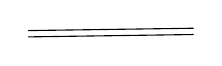
\begin{tikzpicture}[x=1cm,y=1cm]\draw (0,0)--(2.1,0.03);\draw (0,0.08)--(2.1,0.11);\end{tikzpicture}}
\margin{Rem, \unsure{tte} partie modérée $Z$ en pos. rel. \unsure{mod.} avec $X$ et $Y$, l'est aussi avec $X\cap Y$ et $X\underset{\mathrm{mod}}{\cup}Y$}

\uline{Cor} Soit $(X_i)_{i\in I}$ une famille finie de parties fermées modérées mutuellement en pos. \deleted{rel} modérée. Alors $\bigcap_i X_i$ est une partie modérée, et les $X_i$ ont une borne sup. dans l'ens des parties fermées modérées. On a
% slanted
\margin{\uline{Attention} pour une partie \uline{quelc} $A$ de $\mathcal L$, il n'y a \uline{pas} en général d'adh. modérée fermée, i.e. de ``plus petit'' ens f. modéré $X$ tel que $X\supset A$. C'est déjà faux ds le cas standart $L=[0,1]$ ! (Prendre $A=\{0,1/2,1/3\ldots\}$}
\[
\left(\bigcup_{\substack{\mathrm{mod}\\ i}} X_i\right)^{\cdot}\subset\bigcup_i X_i^{\cdot}
\]

\uline{Ex}
\[
[a,b]\underset{\mathrm{mod}}{\cup}[b,c]=[a,c]
\]
mais en général
\[
[a,b]\cup[b,c]\ne[a,c]
\]
(\unsure{prendre|quand} $a$ plus \unsure{c|e} petit élément, $c$ plus grand élément \deleted{\unsure{et}} \unsure{qqconq} \deleted{\unsure{Et en ce} $\unsure{=}$}, $b$ \deleted{\unsure{est}} comp. à tout \inserted{élément de $\mathcal L$.} Si c'est

% pale vertical watermark
\rotatebox{90}{\textsc{\unsure{ra Strong Extra}}}
\scanpage{21}\mspage{20}
vrai pour tt $b$, alors $\mathcal L$ est \unsure{ttt|tt} ordonné. Plus précisém$^{\mathrm t}$, pour que $\mathcal L$ ttt ordonné, il f et s. que pour tt $b\in\mathcal L$, $b$ soit comparable à tt autre élément, ce qui s'écrit
\[
\underbrace{\mathcal L_{\leq b}\underset{\mathrm{mod}}{\cup}\mathcal L_{\geq b}}_{\mathcal L}=\mathcal L_{\leq b}\cup \mathcal L_{\geq b}
\]
\begin{center}\rule{2.5cm}{0.35pt}\end{center}

Partie loc. fermée modérée

\uline{Th} Soi\deleted{\unsure{ent}}t $X\deleted{\unsure{\subset|\supset}},Y$ deux parties fermées modérées, avec $X\supset Y$ (donc $X$ et $Y$ en pos. \unsure{relation|relative} modérée)
\deleted{Considérons les} \deleted{Alors $\exists$ une plus petite partie fermée modérée \inserted{$Z$} contenant $X\setminus Y$.}
Soit
\[
\deleted{\unsure{\complement_X|C_X|\partial X}} C_{\mathrm{mod}}(Y,X)=\left\{x\in X\ \middle|\ 
\begin{aligned}&x\notin Y,\ x\text{ en pos. rel.}\\[-2pt]&\hphantom{x\notin Y,\ x\text{ en }}\text{mod. avec }Y\end{aligned}\right\}
\]
Alors $\exists$ plus petit ens. fermé modéré $Z$ \deleted{tel} \inserted{\unsure{contenant}} \deleted{\unsure{tt|te}} $C_{\mathrm{mod}}(Y,X)$, \deleted{\unsure{a}}\inserted{Ce} $Z$ \inserted{est $\subset X$, et} contient \deleted{\unsure{tt}} partie fermée modérée $T$ de $\mathcal L$ telle que $T\subset X$, $T\cap Y=\emptyset$, $T$ en pos. rel. mod par. \inserted{\unsure{rapt|rel.}} à $Y$, \inserted{De plus} $Z$ est en position modérée avec $Y$.
% slanted
\margin{\uline{On pose} $Z=X\underset{\mathrm{mod}}{\setminus}Y$}

% pale vertical watermark
\rotatebox{90}{\textsc{\unsure{ng Extra Stro}}}
\scanpage{22}\mspage{21}
Si on pose $\deleted{\unsure{S|J}}F=$ frontière relative de $Y$ dans $X$, \deleted{\unsure{c.} F} Alors $F$ est fini, \inserted{modéré,} en pos. mod. p.r. à $Y$, \deleted{\unsure{donc|dans}} $F\subset Z$, \deleted{$\unsure{F\cap Z}$} \deleted{\unsure{est}} $F$ ne \deleted{$\unsure{Z}$} contient pas de pts isolé de $Z$.
\deleted{et on a}
\[
\deleted{\mathrm{Comp}}\ C_{\mathrm{mod}}(Y,X)=C_{\mathrm{mod}}(\deleted{\unsure{Z}}F,Z)
\]
\figure{\tikz{\draw (0,0) .. controls (.07,.02) and (.15,.10) .. (.21,.08) .. controls (.24,-.03) and (.38,-.01) .. (.55,.04) .. controls (.70,.11) and (.74,-.04) .. (.90,-.04) .. controls (1.22,-.05) and (1.33,.05) .. (1.48,.05) .. controls (1.66,-.04) and (1.78,-.08) .. (1.95,-.06) .. controls (2.16,-.05) and (2.27,.08) .. (2.41,.05) .. controls (2.56,-.05) and (2.81,-.05) .. (3.04,.00) .. controls (3.20,.02) and (3.32,.12) .. (3.42,.06) .. controls (3.50,-.08) and (3.80,-.02) .. (4.10,-.01);}}

(9 juin) Soit $\mathcal L$ un tronçon ordonné.

\deleted{Un sous-segment dans \uline{sous-tronçon} \uline{fermé} de $\mathcal L$ est un sous ens de la forme $[a,$}

\textcircled{1} Topologie sur $\mathcal L$ : base d'ouverts les $]a,b[$ (pour $a<b$), $\mathcal L_{<a}$\deleted{\unsure{,}}, $\mathcal L_{>b}$
[NB si $\mathcal L$ n'a pas de plus petit élément (resp. de plus grand élément) on peut omettre les $\mathcal L_{<a}$ (resp. les $\mathcal L_{>b}$). \inserted{Une extrémité de} \deleted{Pour que $\unsure{\{a\}}$ soit} $\mathcal L$ \unsure{—|(} (s'il y en a) est fermé, mais \deleted{fermé, il f et \unsure{suff} s. que}
On fera attention qu'en général, \deleted{les $\unsure{\{a\}}$} \deleted{\unsure{si $a$ est|si $a$ et}} pour $a\in\mathcal L$ $\{a\}$ \uline{n'est pas} \inserted{\uline{néc$^{\mathrm t}$}} \uline{fermé}. Si $\mathcal L$ est l'ens des lieux d'une \deleted{\unsure{segm}} ficelle topologique$^{\ast}$, et alors $\deleted{\unsure{a}}b\in\overline{\{\deleted{\unsure{b}}a\}}$ i.e. $\overline{\{b\}}\subset\overline{\{a\}}$, équivaut à $b\supset a$ (en tt que parties de \unsure{$\mathscr H$|$\mathcal H$|$H$})

% pale vertical watermark
\rotatebox{90}{\textsc{\unsure{Strong Extra}}}
\scanpage{23}\mspage{22}
Il en résulte que $\overline{\{\deleted{\unsure{b}}a\}}=\overline{\{b\}}\Longleftrightarrow a=b$ (donc l'espace top $\mathcal L$ satisfait l'axiome $T_0$, il est ``présobre'' i.e. s'injecte dans le présobrifié) -- je ne sais si c'est
le cas pour tout tronçon, ni si un tronçon, avec sa top. canonique, est sobre (donc, de plus, tte partie fermée \uline{irréductible} aurait un pt générique \dots)
\figure{\begin{tikzpicture}[x=1cm,y=1cm]\draw (0,0)--(1.25,-.03)--(1.56,1)--(3.4,1);\draw (1.18,-.01)--(1.49,1);\end{tikzpicture}}
\margin{\unsure{A|À} voir,}
les ``segment'' $[a,b]$ ne sont pas néc. fermés pour la top. canonique$^{\dagger}$\unsure{,|.}
Ce n'est que lorsque $\mathcal L$ est \uline{tot} ordonné qu'on peut conclure que les pts sont fermés (réciproque ?) et en fait, $\mathcal L$ est $\unsure{=|\simeq}$ \uline{séparé}, et de plus les $[a,b]$, $\mathcal L_{\geq a}$, $\mathcal L_{\leq\deleted{\unsure{b}}a}$ sont fermés.

On peut définir une autre topologie, ayant comme base fondamentale de fermés les $[a,b]$, $\mathcal L_{\geq a}$, $\mathcal L_{\leq a}$ (dont on prend les intersections quelc. de réunions finies, pour avoir tous les fermés)

% pale vertical watermark
\rotatebox{90}{\textsc{\unsure{ng Extra Stro}}}
\scanpage{24}\mspage{23}
Mais maintenant, on est ennuyé, car $]a,b[$ n'a plus envie d'être ouvert !

\deleted{\unsure{ici|on}} On peut bien sûr prendre la topologie borne sup. des deux, ayant comme base d'ouverts

\[
\begin{aligned}
 \mathcal L_{<a},\,\mathcal L_{>a},\quad &]a,b[ && (a<b)\\
 \complement \mathcal L_{\deleted{\unsure{\leq|>}}\geq a},\,\complement \mathcal L_{\leq a},\quad &[a,b] && (a<b)
\end{aligned}
\]

\deleted{De sorte que $]a,b[$ \unsure{est|est un}} \deleted{Sera-t-il vrai, si $a\unsure{\nless|\leq|<}b$, et} \deleted{Mais} \deleted{$b$ n'est pas plus grand élément, que}

Aura-t-on \deleted{$b\in [a,b$}
\[
\begin{aligned}
 \overline{]a,b[}&=[a,b]\quad ?\\
 \overline{\mathcal L_{<a}}&=\mathcal L_{\leq a}\quad ?\quad \text{(si $a$ \deleted{\unsure{n'|est}} n'est pas plus petit élément\unsure{—|)}} \quad \inserted{(a\ne\unsure{o|0}_{L})}\\
 \overline{\mathcal L_{>a}}&=\mathcal L_{\geq a}\quad ?\quad \text{(si $a$ n'est pas plus grand élément ?)}
\end{aligned}
\]

\figure{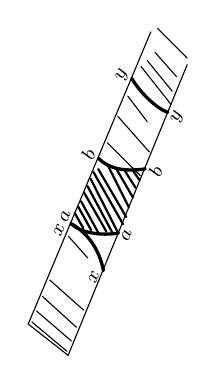
\begin{tikzpicture}[rotate=67,x=.84cm,y=.84cm,line cap=round,line join=round,every node/.style={transform shape,inner sep=1pt,font=\scriptsize}]\draw (.20,.74)--(4.99,.76) (0,0)--(4.75,.06);\draw (0,0)--(.20,.74);\draw[thin] (.05,.04)--(.25,.70) (.22,.04)--(.43,.70) (.44,.05)--(.67,.71) (.72,.05)--(.94,.70) (1.47,.30)--(1.66,.70) (2.93,.06)--(3.19,.71) (3.31,.07)--(3.62,.72) (3.72,.28)--(3.96,.70) (4.10,.05)--(4.45,.69) (4.29,.11)--(4.57,.64) (4.52,.14)--(4.73,.58) (4.84,.10)--(5.08,.69);\draw[very thick] (1.39,.01) .. controls (1.64,.18) and (1.82,.43) .. (1.85,.74) (2.00,.02) .. controls (1.85,.26) and (1.78,.55) .. (1.85,.74) (3.05,.03) .. controls (2.88,.31) and (2.84,.54) .. (2.92,.74) (3.97,.05) .. controls (3.96,.23) and (4.08,.55) .. (4.23,.75);\draw[thick] (1.86,.54)--(2.02,.75) (1.88,.42)--(2.13,.74) (1.89,.31)--(2.22,.73) (1.95,.20)--(2.36,.74) (1.97,.11)--(2.47,.73) (2.01,.04)--(2.59,.73) (2.15,.01)--(2.70,.73) (2.27,.01)--(2.77,.68) (2.42,.03)--(2.87,.56) (2.58,.03)--(2.88,.43) (2.73,.05)--(2.91,.31) (2.86,.04)--(2.96,.20);\node[above] at (1.69,.75) {$x$};\node[above] at (1.92,.75) {$a$};\node[above] at (2.91,.75) {$b$};\node[above] at (4.22,.76) {$y$};\node[left] at (1.38,.10) {$x$};\node[below] at (2.01,.01) {$a$};\node[below] at (3.07,.02) {$b$};\node[below] at (3.96,.03) {$y$};\end{tikzpicture}}
\deleted{\unsure{Donc|D'où}} On est ramené, dans le premier cas, à prouver (p. ex.) $a\in\overline{]a,b[}$, et pour ceci, \inserted{il suffit de voir} \deleted{On} que tte ouvert ``élémentaire'' qui contient $a$, contient un $]a,\varepsilon[$, avec $a<\varepsilon<b$. Mais c'est faux déjà pour un ens. de lieux associé à une ficelle topologique, \deleted{\unsure{en}} [prendre ouvert él. $\complement[x,y]$\unsure{—|.}

% slanted
\margin{Il faut avoir que $a\in\complement[x,y]$ mais $]a,b[\,\subset [x,y]$}

% pale vertical watermark
\rotatebox{90}{\textsc{\unsure{Strong Extra}}}
\scanpage{25}\mspage{24}
Finalement, on travaillera avec la top. définie d'abord (base formée avec les ``intervalles''), et on appellera néanmoins par abus de langage, les $[a,b]$, $\mathcal L_{\leq a}$, $\mathcal L_{\geq b}$ (ainsi que $\mathcal L$) \uline{sous-tronçons} \unsure{ordonnés|ordinaires} (ou \unsure{biordonnés|bien donnés|bien disons|binominés}) ``fermés'', [NB on les suppose non réduits à un pt, i.e.
\[
\deleted{\unsure{[|i}} a<b\quad \text{resp.}\quad a\ne\mathrm{or}(\mathcal L)\quad \text{resp.}\quad \deleted{\unsure{a}}b\ne\mathrm{ex}(\mathcal L)\;]
\]

Un \uline{sous-tronçon \inserted{fermé} large} est une \deleted{sous-tronçon} partie qui est soit un ss-tronçon, soit \unsure{réduit|réduite} à un pt.

Pour une telle partie, $T$, on
% Widely spaced strokes cross the whole lower block, from pose to the last example.
% The close zigzags and local horizontal cancellations show an earlier level of correction.
\deleted{pose}
\[
\begin{aligned}
\deleted{\partial T=}&\deleted{\{t\in T\mid t\in \overline{\mathcal L\setminus T}\}}\quad\text{\deleted{bord}}\\
 &\text{\deleted{\unsure{frontière dans la top.|frontière dans la top}}}\\
 &\text{\deleted{absolu de $T$ $=$ ensemble}}\\
 &\text{\deleted{canonique}}\\
 \deleted{={}\unsure{T\cap\mathcal L|T\cap\overline{\mathcal L}}}&\quad\text{\deleted{fermé de ses extrémités}}\\
 &\deleted{(\mathrm{NB}\ \mathrm{card}\,\partial T\in\{0,1,2\})}
\end{aligned}
\]

\deleted{On voit que pour un tronçon fermé (\uline{NB} non réduit à un pt) on a}

\[
\begin{aligned}
 \deleted{\partial[a,b]=\{a,b\}}&\qquad \deleted{\partial \mathcal L_{\leq a}=\{a\},\quad \partial \mathcal L_{\geq a}=\{a\}}\\
 &\deleted{\partial\mathcal L=\emptyset}
\end{aligned}
\]

% faint vertical paper watermark
\rotatebox{90}{\textsc{\unsure{ng Extra Stro}}}
